\setchapterpreamble[o]{
	\begingroup
	\vspace*{-3cm}\hspace*{-2.56cm}
	\includegraphics[width=\paperwidth,height=8cm,keepaspectratio=false]{images/seaside}
	\vspace*{-1.6cm}
	\addtokomafont{captionlabel}{\bfseries}
	\addtokomafont{caption}{\bfseries}
	\captionsetup{
		type=figure,
		%format=marginemph, 
		%width=\textwidth+\marginparsep+\marginparwidth,
		%indention=2cm,
		%parindent=-2cm,
	}
	\caption[The seaside]{\textbf{By Bushra Feroz - Own work, CC BY-SA 4.0, 
		https://commons.wikimedia.org/w/index.php?curid=68724647}}
	\endgroup
}
% beforeskip=-(figure_height-top_margin)
\RedeclareSectionCommand[beforeskip=-5.1cm]{chapter}
\setchapterpreamble[u]{\margintoc[*-4.5]}

\makeatletter
\renewcommand{\chapterlinesformat}[3]{%
  \@hangfrom{#2}{#3}%
}
\makeatother
\renewcommand*{\chapterformat}{%
  \mbox{\chapappifchapterprefix{\nobreakspace}\thechapter
	\autodot\IfUsePrefixLine{}{\enskip}}}

\chapter{Figures and Tables}
\RedeclareSectionCommand[beforeskip=0cm]{chapter}

\section{Normal figures and tables}

Normal figures and tables can be inserted just like in any standard 
\LaTeX\xspace document. The captions will be positioned in the margins 
thanks to the \verb|floatrow| package. The space between the figure and 
the text can be specified with the following commands:

\begin{verbatim}
	\renewcommand\FBaskip{4pt}
	\renewcommand\FBbskip{4pt}
\end{verbatim}

Here is a picture of Mona Lisa (\reffig{normalmonalisa}), as an example. 
The captions are formatted as the marginnotes; to change the options you 
can use \verb|\captsetup| from the \verb|caption| package.

\begin{figure}[h]
	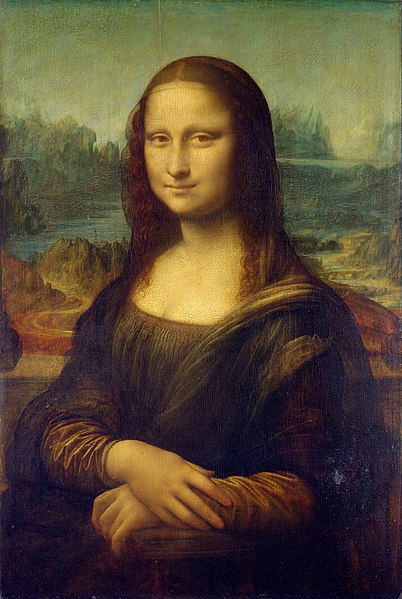
\includegraphics[width=0.4\textwidth]{monalisa}
	\caption[Mona Lisa, again]{It's Mona Lisa again. \blindtext}
	\labfig{normalmonalisa}
\end{figure}

I don't have much to say, so I will just insert some blind text. 
\blindtext

\begin{table}
\begin{tabular}{ |c|c|c|c| } 
\hline
col1 & col2 & col3 \\
\hline
\multirow{3}{4em}{Multiple row} & cell2 & cell3 \\ 
& cell5 & cell6 \\ 
& cell8 & cell9 \\ 
\hline
\end{tabular}
\caption[A useless table]{A useless table.}
\end{table}

\blindtext

\section{Margin figures and tables}

Marginfigures can be inserted with the environment \verb|marginfigure|. 
In this case, the whole picture is confined to the margin and the 
caption is below it. There is also the \verb|margintable| environment, 
of which \reftab{useless} is an example.

\begin{margintable}
\raggedright
\begin{tabular}{ |c|c|c|c| } 
\hline
col1 & col2 & col3 \\
\hline
\multirow{3}{4em}{Multiple row} & cell2 & cell3 \\ 
& cell5 & cell6 \\ 
& cell8 & cell9 \\ 
\hline
\end{tabular}
\caption[Another useless table]{Another useless table.}
\labtab{useless}
\end{margintable}

Marginfigures and tables can be positioned with an optional offset 
command, like so:

\begin{verbatim}
	\begin{marginfigure}[offset]
		\includegraphics{images/seaside}
	\end{marginfigure}
\end{verbatim}

Offset ca be either a measure or a multiple of \verb|\baselineskip| in 
the format \verb|[*5]|.\todo{improve this part} If you are wondering how 
I inserted this orange bubble, have a look at the \verb|todo| package.

\section{Wide figures and tables}

With the environments \verb|figure*| and \verb|table*| you can insert 
figures which span the whole page width. The caption will be positioned 
below.

Now, if you will excuse me, I will add some more blindtext. \blindtext

\blindtext

\begin{figure*}
	\includegraphics{seaside}
	\caption[A wide seaside]{A wide seaside, and a wide caption.
		Credits: By Bushra Feroz - Own work, CC BY-SA 4.0, 
		https://commons.wikimedia.org/w/index.php?curid=68724647.
		\blindtext}
\end{figure*}

%\section{Image before chapter}
%
%It is relatively easy to insert a figure before the chapter title with 
%the help of the \verb|\setchapterpreamble| command. The details are 
%%left 
%to the reader\sidenote{Check the source code for a hint.}.

%Note also that throughout the document I have used different chapter 
%title styles, both to experiment and to show some possibilities. 
%Customising this is quite easy as well.
